\section{Theory}
	Going through the theory in the book \textit{Sensation and perception}, to categorize the different depth cues a tree was made, and to give structure to my essay, I remade a copy of it as seen \autoref{fig:depthCues}, and will utilize this for presenting my findings and answering the topic questions.
	\begin{figure}[H]
		\centering
		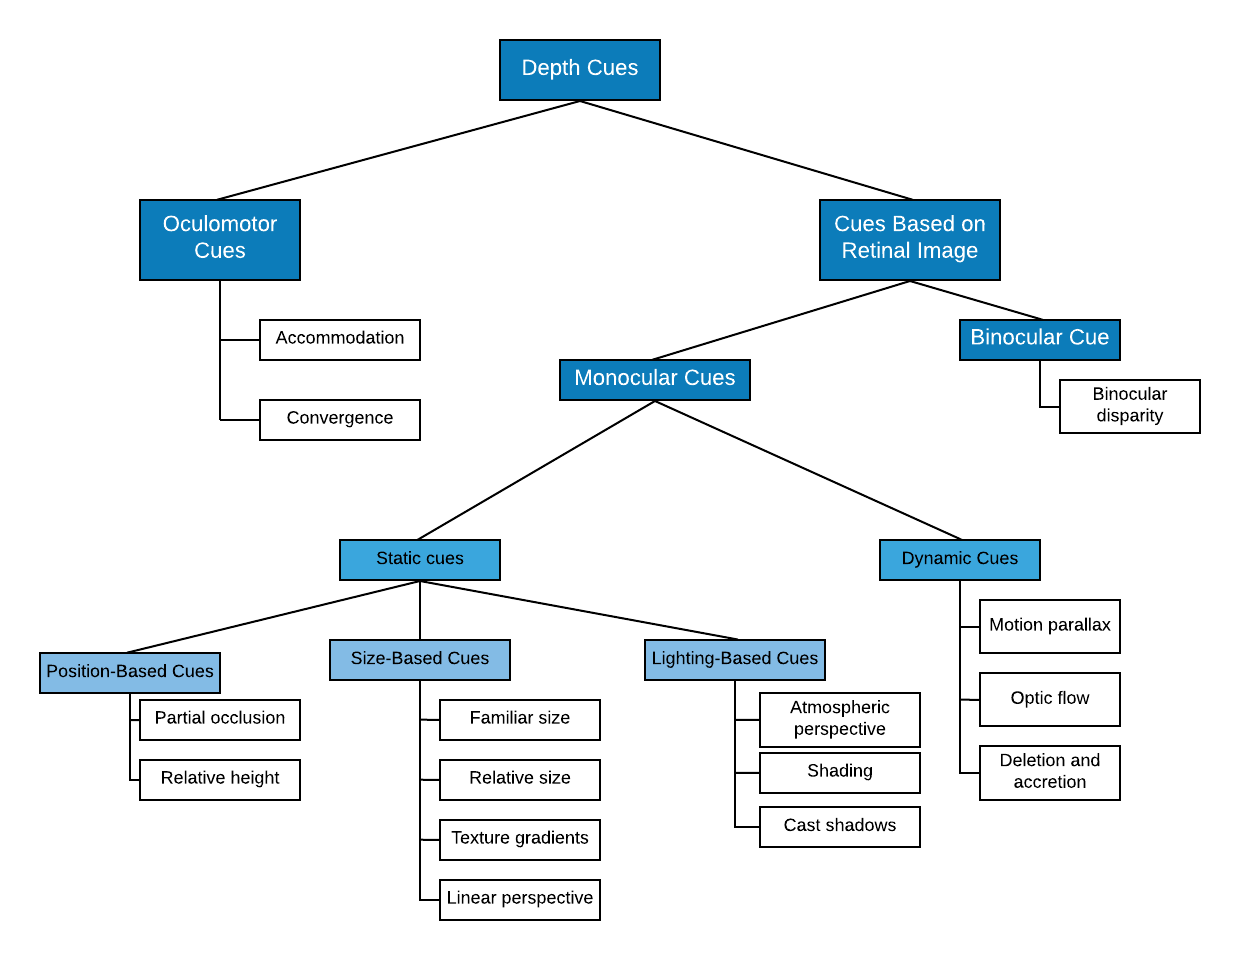
\includegraphics[width=1\linewidth]{figure/depthcues}
		\caption{All the depth cues from the book, Sensation and Perception\citep{sensationPerception}, the figure was made as a copy from the figure on page 195.}
		\label{fig:depthCues}
	\end{figure}
	\subsection{Oculomotor depth cues}
		\subsubsection{Accommodation}
			Focusing on objects, not very much depth data.
		\subsubsection{Convergence}
			Eyes angle moving closer together, objects closer to eyes.
	\subsection{Monocular Depth cues}
		Retinal image information
		\subsubsection{Static cues}
			Cues that require no movement
			%Position
			\paragraph{Partial Occlusion}
				Objects that covers each other
			\paragraph{Relative Height}
				The position of objects in relation to your eye level.
			%Size
			\paragraph{Familiar Size}
				Expectations of objects size, infer depth.
			\paragraph{Relative Size}
				Golf ball size vs basketball size, if they seem identical in size, then the golf ball must be closer.
			\paragraph{Texture Gradients}
				See a texture, that gets smaller, it looks like it is further away.
			\paragraph{Linear Perspective}
				Parallel lines that get closer together, also infer depth.
			%Lighting
			\paragraph{Atmospheric Perspective}
				Due to the air and dust and such, further objects seem less "sharp"
			\paragraph{Shading}
				Sun is natural and expected light, is above, gives shading on everything, gives expectations of depth. figure 6.16.
			\paragraph{Cast shadow}
				Objects casting shadow, gives cue of their depth, due to where the shadow lands, and size of it.
		\subsubsection{Dynamic cues}
			Cues involving movement.
			\paragraph{Motion Parallax}
				Walk left to right, closer objects seem to move faster, than further away objects.
			\paragraph{Optic Flow}
				How objects further away from your focus point moves faster away in relation to your own movement.
			\paragraph{Deletion \& Accretion}
				Deletion = Moving things disappearing behind shit.\\
				Accretion = Moving things appearing from behind shit.
	
		\subsection{Stereopsis}
			The sense of depth, coming from having like two eyes and shit.
		\subsection{binocular disparity}
		Difference between the eyes and shit
		
		\subsection{Stereograms}
		Two images taken with approximately 6 cm (average distance between eyes) separation, produce the feel of depth in the person looking at it.
		
		\subsection{Autostereograms}